\def\solutionMode{TRUE}%
\documentclass[11pt]{article}%
\usepackage{solutions}%
\usepackage{374}%
\usepackage{374_extra}% 
\usepackage{wasysym}
\begin{document}

\noindent\textbf{\LARGE H{}W Solution}\\
\noindent{\textbf{\Course: \CourseName, \Semester}}
\hfill\Version{1.0}%
\\[-0.12cm]
%
\Hr%
\smallskip%

\noindent%
Submitted by:
\begin{compactitem}
    \item \textbf{Yifei Liu}:
    \textbf{yifeil6}
\end{compactitem}
\Hr
\medskip
\SaveIndent%

\begin{questions}[start=1]
    \item \SolutionMP{%
        \begin{questions}
            \item \textbf{False}. FP growth can be as fast as Apriori with certain dataset and min\_sup due to its overhead.

            \item \textbf{False}. Item within an element is unordered.

            \item \textbf{False}. Lies on the margin bound.

            \item \textbf{False}. Most if not all clustering analyses are unsupervised.
            \item \textbf{False}. Zero-shot learning is still supervised.
            \item \textbf{False}. Adding a new edge makes it not minimum for the graph $a$.
            \item Gaussian kernel maps the original data dimension into higher dimension and makes all
            linear-inseperable data linear-seperable.
            \item High intra-cluster similarity and low inter-cluster similarity.
        \end{questions}
    }
\end{questions}
\pagebreak
\begin{questions}[start=2]
    \item \SolutionMP{%
        \begin{questions}
            \item $$s\{hot\ dog, hamburgers\}=\frac{2000}{5000}=0.4,$$
            $$c(hot\ dog\Rightarrow hamburgers)=\frac{s(hot\ dog,\ hamburgers)}{s(hot\ dog)}=\frac{2000}{3000}=\frac{2}{3},$$
            Since $s\{hot\ dog,\ hamburgers\}=0.4>min\_sup=25\%$,

            and $c(hot\ dog\Rightarrow hamburgers)>min\_conf=50\%$,

            $hot\ dog\Rightarrow hamburgers$ is a strong association rule.
            \item $$lift(hot\ dog,\ hamburgers)=\frac{s\{hot\ dog,\ hamburgers\}}{s\{hot\ dog\}\times s\{hamburgers\}}=\frac{2000\times 5000}{3000\times 2500}=\frac{4}{3},$$
            Since $lift(hot\ dog,\ hamburgers)=\frac{4}{3}>1$, they are positively correlated.
            \item $$all\_cnofidence(hot\ dog,\ hamburgers)=\frac{s\{hot\ dog,\ hamburgers\}}{\max\{s\{hot\ dog\},\ s\{hamburgers\}\}}=\frac{\frac{2000}{5000}}{\frac{3000}{5000}}=\frac{2}{3}.$$
            \begin{align*}
                max\_cnofidence(hot\ dog,\ hamburgers)
                 & =\max\big\{\frac{s\{hot\ dog,\ hamburgers\}}{s\{hot\ dog\}},\frac{s\{hot\ dog,\ hamburgers\}}{s\{hamburgers\}}\big\}  \\
                 & =\max\big\{\frac{\frac{2000}{5000}}{\frac{2500}{5000}},\frac{\frac{2000}{5000}}{\frac{3000}{5000}}\big\}=\frac{4}{5}. \\
            \end{align*}
            \begin{align*}
                Kulczynski(hot\ dog,\ hamburgers)
                 & =\frac{1}{2}\Big(\frac{s\{hot\ dog,\ hamburgers\}}{s\{hot\ dog\}}+\frac{s\{hot\ dog,\ hamburgers\}}{s\{hamburgers\}}\Big) \\
                 & =\frac{1}{2}\Big(\frac{\frac{2000}{5000}}{\frac{2500}{5000}}+\frac{\frac{2000}{5000}}{\frac{3000}{5000}}\Big)
                =\frac{1}{2}\times \Big(\frac{4}{5}+\frac{2}{3}\Big)
                =\frac{11}{15}.
            \end{align*}
            \begin{align*}
                cosine(hot\ dog,\ hamburgers)
                 & =\frac{s\{hot\ dog,\ hamburgers\}}{\sqrt{s\{hot\ dog\}\times s\{hamburgers\}}} \\
                 & =\frac{\frac{2000}{5000}}{\sqrt{\frac{2500}{5000}\times \frac{3000}{5000}}}
                =\frac{2\sqrt{30}}{15}.
            \end{align*}
            $$lift(hot\ dog,\ hamburgers)=\frac{4}{3},\text{ as calculated above.}$$
        \end{questions}
    }
\end{questions}
\pagebreak
\begin{questions}[start=3]
    \item \SolutionMP{%
        \begin{questions}
            \item Observe that the largest frequent k-itemset is $\{Bread,\ Cheese,\ Milk\}$ which appears 3 times when $k=3$.
            Then we can compute the confidence based on the given rule template.
            $$c(Bread,Cheese\Rightarrow Milk)=\frac{\frac{3}{4}}{\frac{3}{4}}=1,$$
            $$c(Bread,Milk\Rightarrow Cheese)=\frac{\frac{3}{4}}{\frac{4}{4}}=75\%,$$
            $$c(Cheese,Milk\Rightarrow Bread)=\frac{\frac{3}{4}}{\frac{3}{4}}=1,$$
            Given $min\_conf=80\%$, the result is:
            $c(Bread,Cheese\Rightarrow Milk)\text{ and }c(Cheese,Milk\Rightarrow Bread)$.
            \item Running Apriori algorithm on the trasactions w.r.t customer id, we get the
            largest frequent k-itemset where k=3 being

            $\big\{Dairyland-Milk,Tasty-Pie,Wonder-Bread\big\}$ and

            $\big\{Dairyland-Cheese,Sunset-Milk,Wonder-Bread\big\}$.
        \end{questions}
    }
\end{questions}
\pagebreak
\begin{questions}[start=4]
    \item \SolutionMP{%
        Singletons: $a,b,d$
        \begin{center}
            \begin{tabular}{ |c|c|c|c| }
                \hline
                  & a  & b  & d  \\
                \hline
                a & aa & ab & ad \\
                \hline
                b & ba & bb & bd \\
                \hline
                d & da & db & dd \\
                \hline
            \end{tabular}
            \begin{tabular}{ |c|c|c|c| }
                \hline
                  & a & b    & d    \\
                \hline
                a &   & (ab) & (ad) \\
                \hline
                b &   &      & (bd) \\
                \hline
                d &   &      &      \\
                \hline
            \end{tabular}
        \end{center}
        Scan DB once more $\Rightarrow$ 2-itemset $aa,ab,da$
        \begin{center}
            \begin{tabular}{ |c|c|c| }
                \hline
                2-itemset & -last & -first \\
                \hline
                aa        & a     & a      \\
                \hline
                ab        & a     & b      \\
                \hline
                da        & d     & a      \\
                \hline
            \end{tabular}
        \end{center}
        3-itemset candidates: $aaa,aab,daa,dab$, scan the DB once more $Rightarrow$ 3 itemset $\diameter$
        Now GSP algorithm teminates.
        Result: $a,b,d,aa,ab,da$
    }
\end{questions}
\pagebreak
\begin{questions}[start=5]
    \item \SolutionMP{%
        \includegraphics[scale=0.5]{HW1-5.png}
    }
\end{questions}
\pagebreak
\begin{questions}[start=6]
    \item \SolutionMP{%
        \begin{questions}
            \item 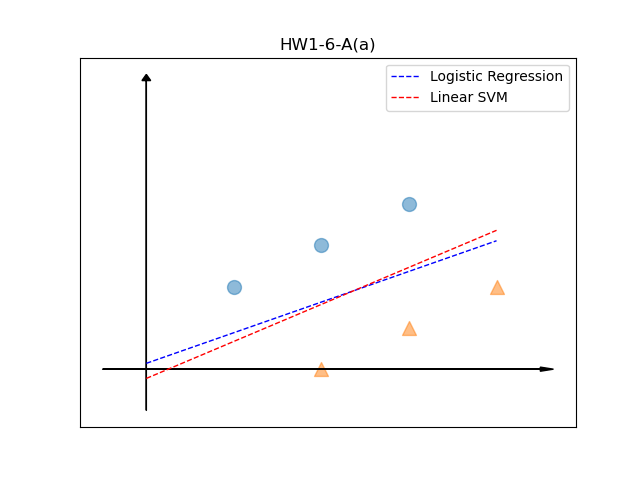
\includegraphics[scale=0.5]{HW1-6-A1.png}
            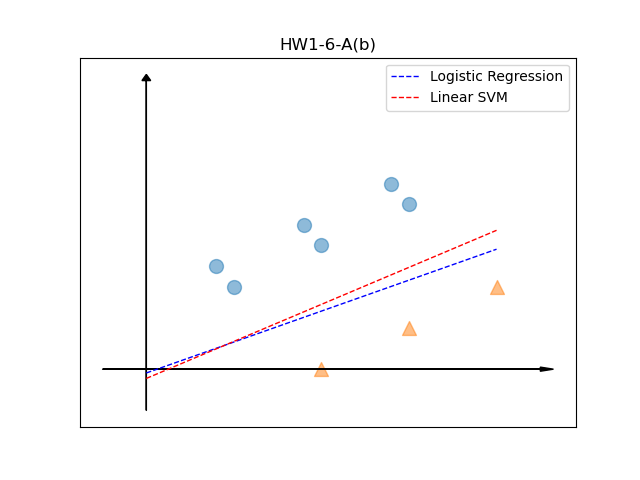
\includegraphics[scale=0.5]{HW1-6-A2.png}

            SVM is more stable to outliers than LR.
            \item Soft-margin SVM: $$argmin_{\{w,b\}}w^tw+\lambda\sum_{i=1}^m\max\{1-y_i(w^tx_i+b),0\}$$
            LR: $$argmin_{\{w,b\}}w^tw+\lambda\sum_{i=1}^m(\ln(1+e^{-w^tx_i}))+(1-y_i)w^tx_i$$

            They share a term $w^tw$ but using different loss function.
            \item Suppose $k_1(X_i,X_j)=\phi_{11}(X_i)^T\phi_{12}(X_j)=\Phi_{1}(X_i \cdot X_j)$ and
            $k_2(X_i,X_j)=\phi_{21}(X_i)^T\phi_{22}(X_j)=\Phi_{2}(X_i \cdot X_j)$

            1.$c_1k_1(X_i,X_j)+c_2k_2(X_i,X_j)=c_1\Phi_{1}(X_i\cdot X_j)+c_2\Phi_{2}(X_i\cdot X_j)$, which is a function of the inner product of $X_i$ and $X_j$.

            2.$k_1(X_i,X_j)k_2(X_i,X_j)=\Phi_{1}(X_i\cdot X_j)\Phi_{2}(X_i\cdot X_j)$, which is a function of the inner product of $X_i$ and $X_j$.

            3.$f(X_i)k_1(X_i,X_j)f(X_j)=f(X_i)\phi_{11}(X_i)^T\phi_{12}(X_j)f(X_j)=\lambda_{1}(X_i)^T\lambda_{2}(X_j)$, where\\
            $\lambda_{k}(X)=f(X)\phi_{1k}(X)$, thus it is a kernel function.
        \end{questions}
    }
\end{questions}
\pagebreak
\begin{questions}[start=8]
    \item \SolutionMP{%
        \begin{questions}
            \item Prove by induction:\\

            \textbf{Base Case:}\\
            $A^2[i,j]=\sum_{t=1}^nA[i,t]A[t,j]$, which represents the number of $t$s s.t.
            there is an edge from $i$ to $t$ and an edge from $t$ to $j$. Thus $A^2[i,j]$ denotes
            the number of $2-hop\ walk$s from $i$ to $j$.\\


            \textbf{Inductive Hypothesis:}\\
            Suppose $A^{k-1}[i,j]$ denotes the number of $\{k-1\}-hop\ walk$ from $i$ to $j$.\\

            \textbf{Inductive Step:}\\
            $A^k[i,j]=\sum_{t=1}^nA^{k-1}[i,t]A[t,j]$, which represents the sum of $W_t,\forall t$ s.t. there is an edge from\\
            $t$ to $j$, where $W_t$ is the number of $\{k-1\}-hop\ walk$s from $i$ to $t$. Thus $A^k[i,j]$ denotes
            the number of $k-hop\ walk$s from $i$ to $j$.
            \item With restart, the similarity of the queried node is much higher than without.
        \end{questions}
    }
\end{questions}
\pagebreak
\begin{questions}[start=9]
    \item \SolutionMP{%
        \begin{questions}
            \item \begin{itemize}
                \item $w_j^t$ is prior distribution of cluster $j$ at step $t$.
                \item $P(x_i|\mu_t^t,\sigma_j^t)$ is the Gaussian distribution that in GMM assumption
                      each cluster follows.

                      $P(x_i|\mu_t^t,\sigma_j^t)=\frac{1}{\sqrt{2\pi (\sigma_j^t)^2}}e^{-\frac{(x_i-\mu_j^t)^2}{2(\sigma_j^t)^2}}$
                \item The denominator is the probability of $x_i$ is clustered in one of the K clusters.
                      Adding it is to find the conditional probability and normalize.
            \end{itemize}
            \item Yes.
            \item Objective function for GMM: $$L=\sum_i\ln(\sum_kw_kp(x_i|\mu_k,\Sigma_k))=
                \sum_i\ln(\sum_kw_k\frac{e^{\frac{-(x_i-\mu_k)^2}{2\sigma_k^2}}}{\sqrt{2\pi\sigma^2}})$$
            We have $\sigma_1^t=\sigma_2^t=\epsilon$, then we have the optimization problem to be
            $argmax_{\{w,\mu,\sigma\}}L$, which is equivalent to
            $argmax_{\{w,\mu\}}\sum_i\epsilon\sum_ke^{\frac{-(x_i-\mu_k)^2}{\epsilon}}$.

            Then we have
            \begin{align*}
                \lim_{\epsilon\to0}\sum_i\epsilon\sum_ke^{\frac{-(x_i-\mu_k)^2}{\epsilon}}
                 & = lim_{\epsilon\to0}\sum_i\frac{\sum_ke^{\frac{-(x_i-\mu_k)^2}{\epsilon}}}{\sum_ke^{\frac{-(x_i-\mu_k)^2}{\epsilon}}}                                             \\
                 & = lim_{\epsilon\to0}\sum_i\frac{\sum_ke^{-\frac{(x_i-\mu_k)^2-\min_k((x_i-\mu_k)^2)}{\epsilon}}}{-\sum_ke^{\frac{(x_i-\mu_k)^2-\min_k((x_i-\mu_k)^2)}{\epsilon}}} \\
                 & = lim_{\epsilon\to0}\sum_i\min_k(x_i-\mu_k)^2                                                                                                                     \\
                 & = \sum_i\lim_{\epsilon\to0}min_k(x_i-\mu_k)^2                                                                                                                     \\
                 & = \sum_i\min_k(x_i-\mu_k)^2
            \end{align*}
            Which is equivalent to the K-Means objective function. $\blacksquare$
        \end{questions}
    }
\end{questions}
\pagebreak
\begin{questions}[start=10]
    \item \SolutionMP{%
        \begin{questions}
            \item The eigenvector is \textbf{1}. $L_{ii}=-A_{ii}+\sum_jA_{ij}$ and $L_{ij}=-A_{ij},i\neq j$.

            Thus solution for $Lx=\lambda x=\textbf{0}$ is $x=\textbf{1}$.

            We cannot use it as all the values are the same.
        \end{questions}
    }
\end{questions}
\end{document}

%%%%%%%%%%%%%%%%%%%%%%%%%%%%%%%%%%%%%%%%%%%%%%%%%%%%%%%%%%%%%%%%%%%%%%%%
%%%%%%%%%%%%%%%%%%%%%%%%%%%%%%%%%%%%%%%%%%%%%%%%%%%%%%%%%%%%%%%%%%%%%%%%
%%%%%%%%%%%%%%%%%%%%%%%%%%%%%%%%%%%%%%%%%%%%%%%%%%%%%%%%%%%%%%%%%%%%%%%%
